% Compile from the project root with tectonic COURSE_PROJECT_SLIDES.tex.
% Rebuild figures with python scripts/build_slide_assets.py.
% The 17 numbered frames have a target running time of 18 minutes.
% Speaker notes are embedded with \note{} and hidden in the audience PDF.
\documentclass[aspectratio=169,11pt]{beamer}
\usepackage[T1]{fontenc}
\usepackage{lmodern,amsmath,amssymb,booktabs}
\usepackage{tikz}
\usetikzlibrary{positioning,arrows.meta,calc}
\usefonttheme{professionalfonts}
\definecolor{navy}{HTML}{16364A}
\definecolor{teal}{HTML}{007F83}
\definecolor{orange}{HTML}{C45A13}
\definecolor{muted}{HTML}{576574}
\setbeamercolor{normal text}{fg=navy,bg=white}
\setbeamercolor{structure}{fg=teal}
\setbeamercolor{frametitle}{fg=navy}
\setbeamercolor{block title}{fg=white,bg=navy}
\setbeamercolor{block body}{fg=navy,bg=navy!5}
\setbeamerfont{frametitle}{size=\Large,series=\bfseries}
\setbeamerfont{title}{size=\LARGE,series=\bfseries}
\setbeamertemplate{navigation symbols}{}
\setbeamertemplate{itemize items}[circle]
\setbeamersize{text margin left=8mm,text margin right=8mm}
\setbeamertemplate{footline}{%
  \hspace{8mm}\textcolor{muted}{\scriptsize\insertsectionhead}
  \hfill\textcolor{muted}{\scriptsize\insertframenumber/\inserttotalframenumber}
  \hspace{8mm}\vspace{3mm}}
\setbeamertemplate{frametitle}{\vspace{3mm}\insertframetitle\par\vspace{2mm}}
\setbeameroption{hide notes}
\newcommand{\norm}[1]{\lVert #1\rVert_2}
\newcommand{\tf}{f_\phi}
\newcommand{\source}[1]{\par\vfill{\color{muted}\tiny #1}}
\title{Stability and Information Sensitivity\\in Transformer In-Context Inverse Learning}
\author{Fei Zhang}
\institute{University of Waterloo\\CS 886}
\date{November 2026}

\begin{document}
\section{Motivation}

% 1. 0:00--0:30
\begin{frame}[plain]
\vfill
{\usebeamerfont{title}\inserttitle\par}
\vspace{6mm}
{\large Fei Zhang\par}
\vspace{2mm}
{\color{muted}University of Waterloo\quad CS 886\par}
\vspace{8mm}
{\color{teal}\large How much should one observation change a learned estimate?}
\vfill
\note{Target time 30 seconds, cumulative 0:30.
Today I will discuss how a Transformer learns from a small context when some
observations are much more informative than others. Our setting lets us
calculate which parameter directions the observations identify. The talk
connects an architectural stability proof to a recovery limitation, then
tests the trained models on controlled changes to those observations.}
\end{frame}

% 2. 0:30--1:35
\begin{frame}{One observation can identify a missing direction}
\begin{columns}[T,onlytextwidth]
\column{.47\textwidth}
{\large An affine inverse problem}
\[
 y=a+bx
\]
\[
 \underbrace{(0,a),\ldots,(0,a)}_{m-1\text{ observations}}
\]
The shared records identify \(a\).
\column{.47\textwidth}
{\large One identifying record}
\[
 (h,a+hb),\qquad h\ne0
\]
This record identifies \(b\).
\[
 (h,a+hb')\quad\Longrightarrow\quad b'
\]
\end{columns}
\vspace{5mm}
\begin{block}{Research question}
Can a Transformer remain stable while responding enough to an observation
that determines the correct answer?
\end{block}
\note{Target time 65 seconds, cumulative 1:35.
Start with a line. Repeating the input zero tells us the intercept precisely,
but it never supplies the slope. A single observation at a nonzero input
supplies that missing direction. If we change that observation to one from
a different line with the same intercept, the correct slope changes even
though almost the entire context is identical. This example motivates a
distinction between a record that merely adds another sample and one that
changes which parameter is identified. We want to understand whether a
trained Transformer makes a sufficiently large response in the second case.}
\end{frame}

% 3. 1:35--2:30
\begin{frame}{From a stability theorem to an inverse-learning test}
\begin{itemize}
\setlength{\itemsep}{4mm}
\item Li et al.\ (ICML 2023) relate Transformer ICL to algorithmic stability.
\item We audit stability for the implemented \textbf{mean-pooled encoder}.
\item A valid inverse problem lets us construct records that identify
otherwise missing cost directions.
\item Controlled interventions measure the trained model's response and recovery.
\end{itemize}
\source{Li, Ildiz, Papailiopoulos and Oymak (2023). The generic recovery lower bound uses the triangle inequality.}
\note{Target time 55 seconds, cumulative 2:30.
The motivating paper views a Transformer as an algorithm operating on its
context. It proves stability for a particular query-token architecture.
Our contribution in this course project is to verify a related claim for
the set encoder we actually implemented, and to examine the recovery
consequences through an explicit optimization model. We use established
proof tools. The concrete dispatch construction and the matched tests
make their implications observable. I will first explain the setup,
then the proofs, and use the results to assess how much the trained
model responds to the relevant information.}
\end{frame}

\section{Methodology}
% 4. 2:30--3:35
\begin{frame}{Optimal dispatch produces interpretable observations}
\begin{columns}[T,onlytextwidth]
\column{.53\textwidth}
\[
\min_{\substack{x_1+x_2=d\\0\le x_i\le1}}
\sum_{i=1}^{2}\left(a_i x_i+\frac12b_i x_i^2\right)
\]
\vspace{2mm}
\(\theta=(a_1,b_1,a_2,b_2)\) is fixed within a task.
\[
a_i\in[1,1.65],\qquad b_i\in[0.8,2]
\]
We observe demand, optimal outputs, price and bound statuses.
\column{.43\textwidth}
{\large KKT describes the information}
\[
a_i+b_ix_i-\lambda
\begin{cases}
=0 & \text{interior},\\
\ge0 & \text{lower bound},\\
\le0 & \text{upper bound}.
\end{cases}
\]
Two distinct interior outputs identify a unit's two cost coefficients.
\end{columns}
\source{Synthetic two-generator economic dispatch. Positive quadratic coefficients give a unique optimal dispatch.}
\note{Target time 65 seconds, cumulative 3:35.
We use two generators with quadratic costs and known unit capacities.
Every task has a new set of four cost coefficients, and each demand
produces an optimal dispatch and market price. At an interior output,
the price equals the derivative of cost. That is exactly an affine
regression equation. A generator at a bound contributes a one-sided
constraint. We can therefore tell whether a context uniquely identifies
the parameters, whether its linear equations are poorly conditioned,
or whether several parameter values remain compatible. The network
is trained to infer costs from these market observations.}
\end{frame}

% 5. 3:35--4:35
\begin{frame}{A frozen Transformer estimates the task parameters}
\begin{center}
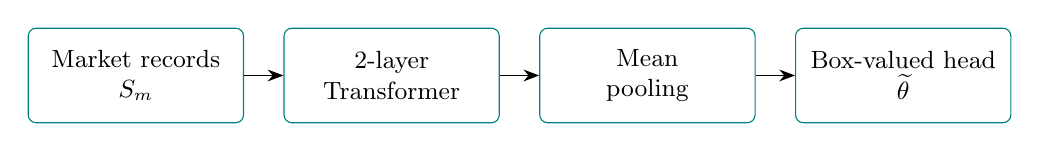
\begin{tikzpicture}[node distance=5mm,
    stage/.style={draw=teal,rounded corners=1mm,align=center,minimum height=12mm,
                  text width=25mm,font=\small},
    >={Stealth[length=2mm]}]
\node[stage] (input) {Market records\\\(S_m\)};
\node[stage,right=of input] (encoder) {2-layer\\Transformer};
\node[stage,right=of encoder] (pool) {Mean\\pooling};
\node[stage,right=of pool] (output) {Box-valued head\\\(\widetilde\theta\)};
\draw[->] (input)--(encoder);
\draw[->] (encoder)--(pool);
\draw[->] (pool)--(output);
\end{tikzpicture}
\end{center}
\vspace{4mm}
\begin{itemize}
\setlength{\itemsep}{2mm}
\item Width 64, four heads, residual blocks, LayerNorm and ReLU.
\item No positional embeddings, zero dropout, unmasked full attention.
\item Supervised training across tasks. Weights stay fixed on unseen tasks.
\end{itemize}
\vspace{3mm}
\textbf{Formulation}\quad Context-conditioned, supervised amortized inverse estimation.
\source{Li et al.\ use a designated query response. Here the output is the latent task parameter vector.}
\note{Target time 60 seconds, cumulative 4:35.
Each observation contributes ten features: four scaled continuous
quantities and two three-way status encodings. The encoder processes
the set, and mean pooling produces one vector. A bounded output head
maps it into the cost box. Training uses known synthetic costs as
labels across source tasks. At test time the network reads records
from new tasks with no parameter update. This makes the connection
to ICL precise: adaptation occurs through context. Our task-level
parameter readout differs from the query-conditioned prediction
used by the reference paper, and the stability proof must account
for the actual pooling operation.}
\end{frame}

% 6. 4:35--5:30
\begin{frame}{Theorem 1 gives a worst-case replacement bound}
\begin{block}{Fixed mean-pooled Transformer}
For finite weights and depth, bounded inputs and positive LayerNorm
epsilon, there is a finite \(C\), independent of \(m\), such that
\[
\boxed{\norm{\tf(S_m)-\tf(S_m')}\le\frac{C}{m}}
\]
whenever the two contexts differ in one record.
\end{block}
\vspace{3mm}
\begin{itemize}
\setlength{\itemsep}{2mm}
\item Full attention and the set readout are part of the assumptions.
\item \(C\) depends on the trained weights and input bounds.
\item The theorem holds in exact arithmetic over the bounded input domain.
\end{itemize}
\note{Target time 55 seconds, cumulative 5:30.
The first theorem is uniform over neighboring bounded contexts.
The architecture has fixed depth and the same fixed parameters at all
lengths. The proof establishes existence of a finite constant with
no dependence on context length. The constant can nevertheless be
extremely large, which matters when we later compare this theorem
with observed sensitivities. The rate is about worst-case behavior
as length changes. Our experiments estimate averages under particular
replacement protocols, so we will compare them with that scope in mind.}
\end{frame}

% 7. 5:30--7:00
\begin{frame}{Proof of Theorem 1 through bounded attention}
\small
At one layer let \(e_i=\norm{h_i-h_i'}\) and
\(\displaystyle \bar e=\frac1m\sum_i e_i\).
\vspace{2mm}
\begin{enumerate}
\setlength{\itemsep}{2mm}
\item One changed input row gives \(\bar e_0\le A/m\).
\item Bounded query and key vectors give \(|s_{ij}|,|s_{ij}'|\le B\), hence
\[
 p_{ij}\le\frac{e^{2B}}m.
\]
\item The softmax Jacobian is \(\operatorname{diag}(p)-pp^\top\).
Its \(j\)-th absolute column sum is at most \(2p_j\), giving
\[
\|p_i-p_i'\|_1
 \le 2e^{2B}(c_q e_i+c_k\bar e).
\]
\item Changing weights and values, then averaging rows, gives
\[
 \frac1m\sum_i\norm{\operatorname{Attn}_i(H)-\operatorname{Attn}_i(H')}
 \le L_{\rm att}\bar e.
\]
\end{enumerate}
\source{\(c_q,c_k,L_{\rm att}\) depend on fixed weight and hidden-state norm bounds, not on \(m\).}
\note{Target time 90 seconds, cumulative 7:00.
The useful quantity is the average difference across rows.
Immediately after embedding, only one row has changed, so its
contribution is diluted by one over the context length.
Attention mixes rows, and we need to show that mixing preserves
this average bound. Bounded scores limit each softmax probability
to a constant divided by m. The softmax Jacobian lets us control
how the probabilities change as queries and keys change.
There is a local term for the changed query row and an average
term for the changed keys. When we average all output rows,
both terms become a fixed multiple of the average input difference.
The same argument controls the change in the value vectors.
The constants can include an exponential in the score bound,
but they have no dependence on m.}
\end{frame}

% 8. 7:00--8:15
\begin{frame}{Residual blocks and pooling preserve the rate}
\begin{columns}[T,onlytextwidth]
\column{.49\textwidth}
{\large Rowwise maps}
\small
\[
L_{\rm LN}\le\frac{\|\gamma\|_\infty}{\sqrt{\eta}},
\qquad \eta>0.
\]
\[
L_{\rm FF+res}\le1+\|W_2\|\|W_1\|.
\]
Each layer multiplies \(\bar e\) by a finite constant.
\column{.47\textwidth}
{\large Pooling and readout}
\small
\[
\left\|\frac1m\sum_i(h_i-h_i')\right\|_2\le\bar e.
\]
\[
L_{\rm head}\le
\frac{\|\operatorname{diag}(\mathrm{span})\|
      \|W_{\rm head}\|}{4}.
\]
Thus \(\displaystyle C=A\,L_{\rm head}\prod_{\ell=1}^{L}L_\ell\).
\end{columns}
\vspace{5mm}
\textcolor{orange}{Measured norm substitution gives
\(\log_{10} C\approx616\)--\(709\) for the original checkpoints.}
\source{Full softmax and LayerNorm derivative arguments are in the report appendix. Matrix norms are Euclidean operator norms.}
\note{Target time 75 seconds, cumulative 8:15.
The remaining operations act row by row, so a Lipschitz bound
on each row gives the same bound on the row average.
LayerNorm needs positive epsilon. Its derivative is bounded by
the maximum gain divided by the square root of epsilon.
The feedforward block and its residual have a finite product bound.
After a fixed number of layers, averaging the states cannot exceed
the average of their differences. The sigmoid head contributes
another finite factor. This completes the proof.
We also substituted weight-based norm bounds into the formula.
The resulting constants are huge, so they establish a rate and
an eventual restriction, while the output-box diameter is tighter
over the measured lengths.}
\end{frame}

% 9. 8:15--9:40
\begin{frame}{Theorem 2 gives the response required for recovery}
Let \(D=\norm{\theta-\theta'}\) for two contexts differing in one record.
Suppose both recovery errors are at most \(\epsilon\).
\begin{align*}
D
&\le \norm{\theta-f(S)}
  +\norm{f(S)-f(S')}
  +\norm{f(S')-\theta'}\\
&\le 2\epsilon+\norm{f(S)-f(S')}.
\end{align*}
\[
\boxed{\norm{f(S)-f(S')}\ge D-2\epsilon}
\]
\vspace{2mm}
Combining with \(C/m\) replacement stability gives
\[
\boxed{\epsilon\ge\frac12\left(D-\frac Cm\right)_+.}
\]
\small\textcolor{orange}{The lower bound is nonzero only when \(m>C/D\).}
\source{The triangle inequality applies to any estimator. The encoder-specific ingredient is its upper bound.}
\note{Target time 85 seconds, cumulative 9:40.
Now take two contexts whose correct parameter vectors differ.
If the estimator is accurate on both, the two predictions have
to be separated. To prove this, go from the first target to its
prediction, then to the second prediction, and finally to the
second target. The two endpoint errors account for at most twice
epsilon, leaving a required change of D minus twice epsilon.
If an independent stability bound limits that change to C over m,
one endpoint must have error at least the displayed lower bound.
This is a general deterministic argument. The project makes it
relevant to the Transformer by supplying its architecture bound
and a pair of valid records inside our task domain.}
\end{frame}

% 10. 9:40--11:00
\begin{frame}{Two dispatch tasks differ only in one clearing price}
\begin{center}
\begin{tabular}{lcc}
\toprule
& Task A & Task B\\
\midrule
Costs of each generator \((a_i,b_i)\)&\((1.6,1.0)\)&\((1.2,1.8)\)\\
Shared record at \(d=1\)&\((0.5,0.5,2.10)\)&\((0.5,0.5,2.10)\)\\
Focal record at \(d=1.6\)&\((0.8,0.8,2.40)\)&\((0.8,0.8,2.64)\)\\
\bottomrule
\end{tabular}
\end{center}
\vspace{2mm}
\begin{itemize}
\setlength{\itemsep}{2mm}
\item Each record lists \((x_1,x_2,\lambda)\). Both units are interior.
\item Repeat the shared record \(m-1\) times, then append the focal record.
\item Two distinct outputs identify each cost. \(D=\sqrt{1.6}\) stays fixed.
\end{itemize}
\vspace{2mm}
\textcolor{teal}{As \(m\) grows, a fixed encoder faces a worst-case error floor \(D/2\).}
\note{Target time 80 seconds, cumulative 11:00.
Here is the actual optimization construction.
Within each task the two units have identical costs, so symmetry
and strict convexity give equal dispatch. At demand one, each
unit produces one half and both cost curves have marginal cost
2.1. At demand 1.6 each produces 0.8, and the prices differ.
The slope can be solved from the two prices and two outputs,
then the intercept follows. Thus each endpoint is identifying.
As we add copies of the shared record the targets stay a fixed
distance apart. The architectural upper bound eventually forces
one prediction to have a substantial error. This is a worst-case
family with exact repetitions. The ordinary experiments use
new observations from the same task, so their correct target stays fixed.}
\end{frame}

% 11. 11:00--11:50
\begin{frame}{The experiments measure response and recovery together}
\begin{columns}[T,onlytextwidth]
\column{.48\textwidth}
{\large Common protocol}
\begin{itemize}
\setlength{\itemsep}{2mm}
\item Three seeds.
\item 1,536 source tasks for D and G.
\item 96 validation and 128 unseen tasks per seed.
\item Test weights stay fixed.
\end{itemize}
\column{.48\textwidth}
{\large Two metrics}
\[
\begin{aligned}
E&=\frac{\norm{f(S)-\theta}}{\norm{\theta}},\\[2mm]
\Delta&=\norm{f(S)-f(S')}.
\end{aligned}
\]
Ordinary replacements keep the task fixed.

\vspace{3mm}
The identifying pair changes the true task.
\end{columns}
\vspace{3mm}
\footnotesize Baselines: norm-controlled Transformer, DeepSets, ridge and sufficient-statistics MLP.

All predictions are evaluated before KKT correction.
\source{Splits are by cost task. Error bars in the following plots show SD across three seed means.}
\note{Target time 50 seconds, cumulative 11:50.
We train and evaluate using disjoint parameter tasks, so test
contexts come from unseen costs. Three seeds provide independent
training and task draws. I will report relative Euclidean recovery
error and absolute Euclidean prediction change. They have different
units and serve different purposes. Architecture stability uses
valid same-task replacements. The cross-task construction uses
two different correct answers. Reading the sensitivity together
with its protocol and the recovery error is essential to interpreting
each plot.}
\end{frame}

\section{Results}
% 12. 11:50--12:55
\begin{frame}{Transformer has lower sensitivity and recovery error in D}
\begin{center}
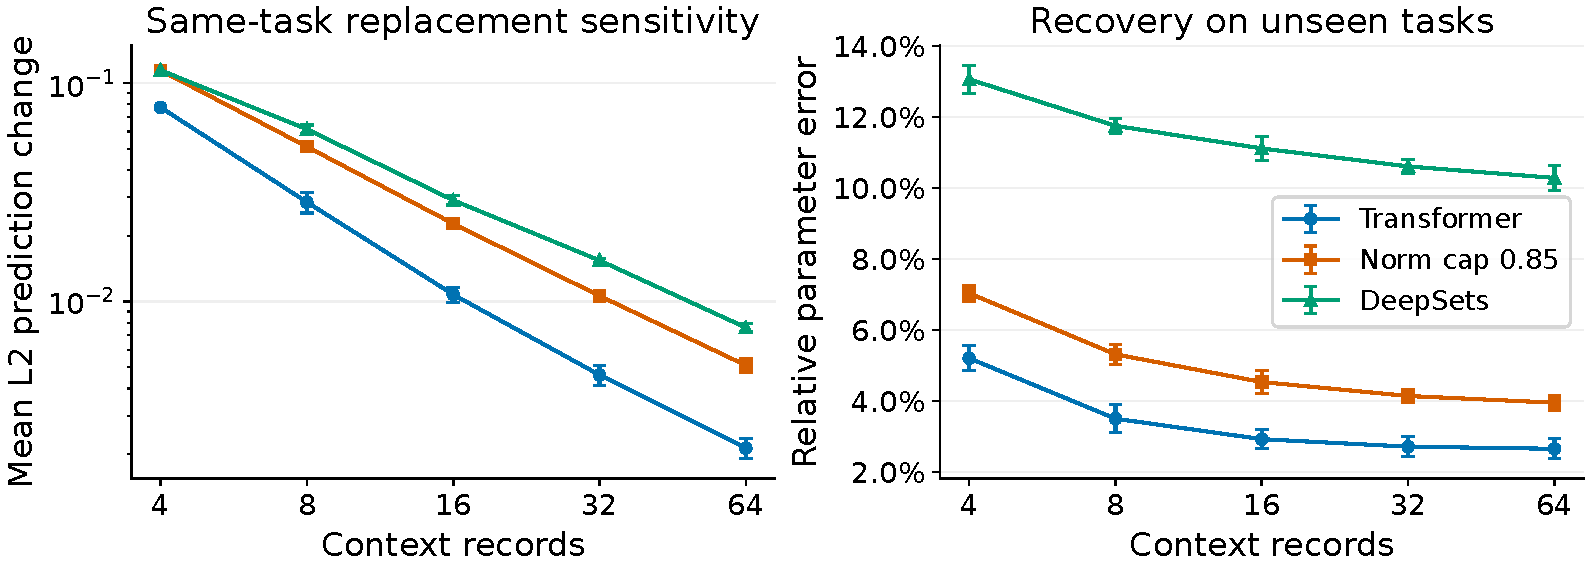
\includegraphics[width=.97\textwidth]{results/presentation/architecture.pdf}
\end{center}
\vspace{-1mm}
\small At \(m=64\), relative errors are
\textbf{2.65\%}, 3.95\% and 10.28\% for Transformer, norm cap and DeepSets.
\source{Experiment D. Four valid same-task replacement trials per task and length.}
\note{Target time 65 seconds, cumulative 12:55.
Both plots show the same three architectures trained under the
same schedule. Average replacement sensitivity falls as context
length grows, and the original Transformer is the least sensitive
in these measurements. It also has the lowest recovery error
at each length. The norm-controlled model does worse under this
schedule, even though the cap bounds part of the worst-case
constant. That is compatible with the theory because training
changes the remaining maps and these are sampled average
responses. At length 64, the original Transformer's error is
2.65 percent, compared with 3.95 for the constrained version
and 10.28 for DeepSets.}
\end{frame}

% 13. 12:55--13:55
\begin{frame}{Unique identification can coexist with poor learned recovery}
\begin{center}
\begin{tabular}{lrrr}
\toprule
Context at \(m=16\)&Minimum Gram eigenvalue&Set diameter&TF error\\
\midrule
Well-conditioned&\(0.03257\)&0&2.90\%\\
Nearly redundant&\(3.72\times10^{-6}\)&0&13.65\%\\
Mixed&\(0.02429\)&0&3.72\%\\
Boundary-heavy&0&1.056&17.64\%\\
\bottomrule
\end{tabular}
\end{center}
\vspace{4mm}
\[
H_i=\frac1m\sum_{t:\,s_{it}=\mathrm{int}}u_{it}u_{it}^{\top},
\qquad u_{it}=(1,x_{it})^\top.
\]
\small The eigenvalue is \(\min_i\lambda_{\min}(H_i)\).
Interior contexts share mean demand; their output spreads differ.
\source{Experiment F. Diameter refers to the boxed KKT-admissible parameter set. Values are seed means.}
\note{Target time 60 seconds, cumulative 13:55.
The first three contexts uniquely determine the cost parameters
in the exact model, as shown by their zero admissible diameter.
Yet nearly redundant contexts give much worse Transformer error.
Their equations use almost the same output repeatedly, producing
a very small minimum Gram eigenvalue. This is a full-rank but
poorly conditioned design. Boundary-heavy contexts add a second
difficulty: a nontrivial set of compatible costs. The task parameters
are matched across regimes, but the status restrictions and
the spread of demand cannot all be held fixed. The first two
interior regimes do share exactly the same mean demand.}
\end{frame}

% 14. 13:55--14:55
\begin{frame}{The same focal price edit has a larger effect at high leverage}
\begin{columns}[c,onlytextwidth]
\column{.68\textwidth}
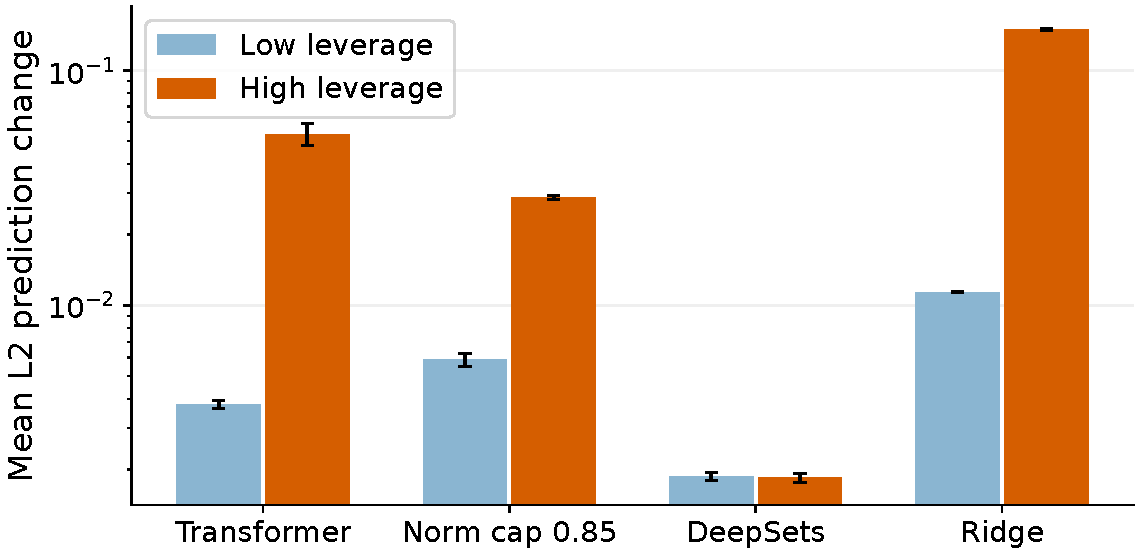
\includegraphics[width=\linewidth]{results/presentation/matched_response.pdf}
\column{.29\textwidth}
\small
Fixed focal record and price displacement.

\vspace{4mm}
Different context backgrounds.

\vspace{4mm}
\textbf{High / low response}
\[
\text{Transformer}\quad14.1\times
\]
\[
\text{Ridge}\quad13.1\times
\]
\end{columns}
\source{Experiment G. Price changes from \(\lambda-0.01\) to \(\lambda+0.01\).
Mean focal leverage is 0.999 versus 0.133.}
\note{Target time 60 seconds, cumulative 14:55.
We now hold the edited observation and the magnitude of the price
change fixed. What changes is the background: most other observations
can be clustered, or spread across the interior interval.
This changes the focal record's statistical leverage.
The original Transformer reacts about fourteen times more strongly
under the high-leverage background. Ridge has a similar ratio.
But the absolute Transformer response is smaller, and DeepSets
has almost no corresponding ratio in this experiment.
This supports information-dependent response at the output.
The interventions leave the internal attention computation unresolved.}
\end{frame}

% 15. 14:55--15:55
\begin{frame}{The identifying response is still too small for accurate recovery}
\begin{columns}[c,onlytextwidth]
\column{.68\textwidth}
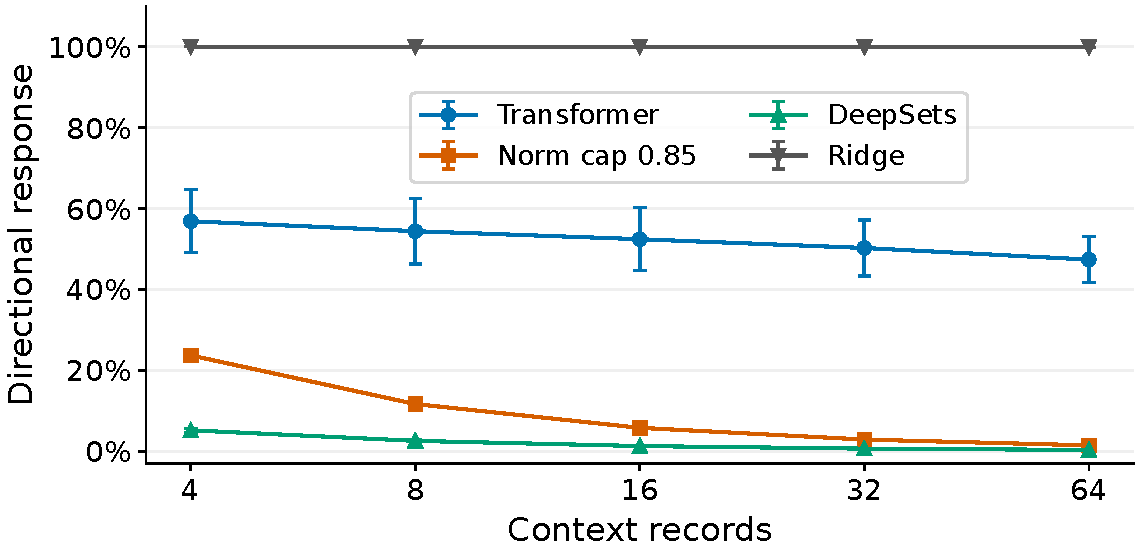
\includegraphics[width=\linewidth]{results/presentation/identifying_response.pdf}
\column{.29\textwidth}
\small
At \(m=64\)
\[
r_{\rm TF}=47.4\%
\]
\[
r_{\rm ridge}=99.9\%
\]
Larger TF endpoint error
\[
0.432.
\]
\end{columns}
\[
\small r=\frac{\langle f(S')-f(S),\,\theta'-\theta\rangle}
                    {\norm{\theta'-\theta}^{2}}.
\]
\source{Experiment G. Valid cross-task pair with \(D=\sqrt{1.6}\). Euclidean endpoint error is in parameter units.}
\note{Target time 60 seconds, cumulative 15:55.
This is the pair from the theoretical construction.
The horizontal reference at one hundred percent means that the
predicted difference recovers the true difference along its direction.
The original Transformer has a substantial response, but it reaches
only 47.4 percent at length 64. Its larger endpoint error averages
0.432. Ridge almost fully recovers the target difference.
The constrained model and DeepSets react much less as the
shared context grows. The original Transformer's response at these
lengths is still compatible with a C over m bound whose constant
is very large. This plot illustrates the recovery requirement
at finite length.}
\end{frame}

% 16. 15:55--17:00
\begin{frame}{Task-count gains depend on the training budget}
\begin{center}
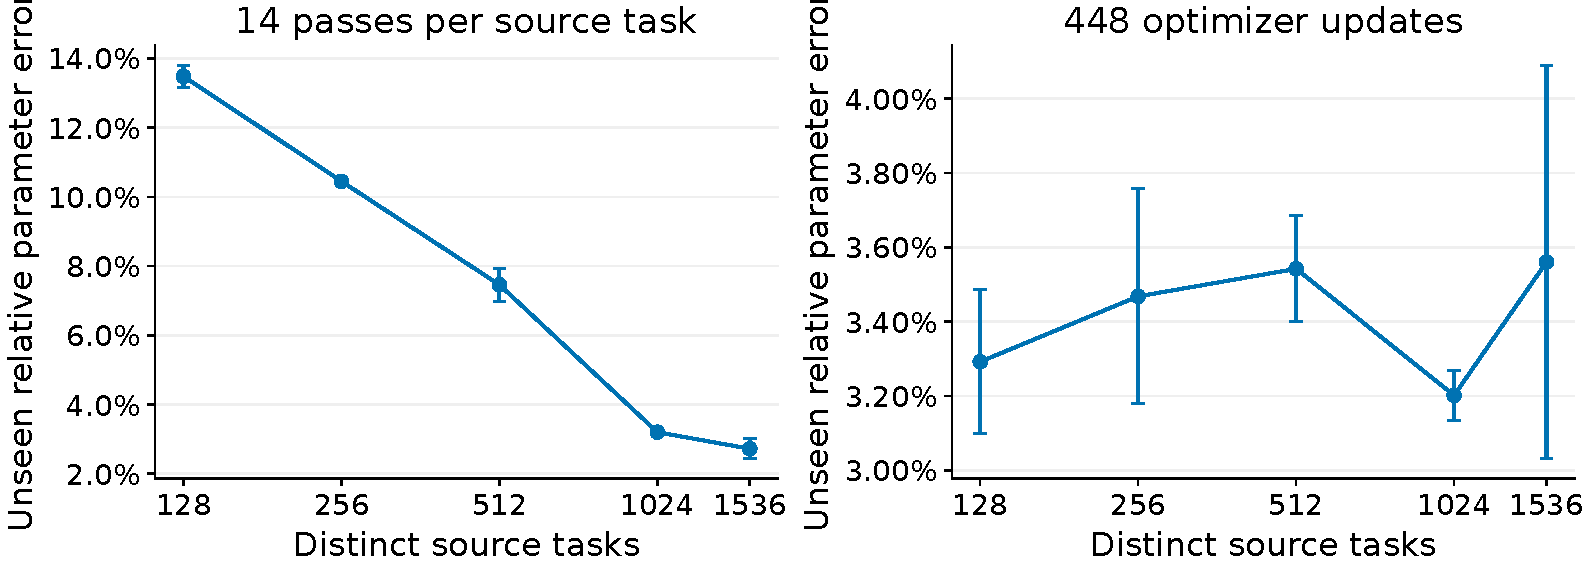
\includegraphics[width=.97\textwidth]{results/presentation/transfer.pdf}
\end{center}
\small The equal-pass sweep spends 56--672 updates as source-task count grows.

\source{Experiment E, evaluation context length 32. Under 448 updates, target error is nonmonotonic across task counts.}
\note{Target time 65 seconds, cumulative 17:00.
The left panel initially suggests that many source tasks improve
transfer substantially. However, keeping passes per task fixed
also increases total optimizer updates as the dataset grows.
The right panel controls the number of updates and yields much
closer, nonmonotonic errors. A later control also fixed training
context length, batch size, record presentations and checkpoint
time; its task-count trend remained nonmonotonic.
Thus the source-task distribution and optimization budget both
matter, while a benefit of task count alone remains unresolved
in this experiment. This is a limitation on the empirical
generalization conclusion, even though a supporting task-level
covering-number bound is available.}
\end{frame}

\section{Conclusion}
% 17. 17:00--18:00
\begin{frame}{Recovery requires enough response to identifying information}
\begin{enumerate}
\setlength{\itemsep}{4mm}
\item A fixed mean-pooled Transformer has a \(C/m\) replacement bound.
\item Accuracy on two tasks distinguished by one record requires a response
of at least \(D-2\epsilon\).
\item The trained model responds to context leverage, but can recover only
part of the identifying parameter difference.
\end{enumerate}
\vspace{5mm}
{\color{orange}Limits}\quad
Loose constants, repeated-demand stress cases, three seeds and two generators.
\vspace{4mm}
{\color{teal}\large Evaluation should connect sensitivity, information and recovery.}
\note{Target time 60 seconds, cumulative 18:00.
The theoretical upper bound and the recovery lower bound concern the
same predictor, but they reveal different requirements.
We verified the architecture-level rate and gave a valid dispatch
family where one observation identifies a cost direction.
The experiments then showed that the trained Transformer changes
its behavior with context information, while its response can
still be insufficient to recover the correct difference.
The finite-sample conclusions are limited by the task model,
the number of seeds, the training schedule, and very loose
worst-case constants. The course-project contribution is the
connection between the guarantee, the explicit construction,
and controlled measurements of response and accuracy.}
\end{frame}

\appendix
\setbeamertemplate{footline}{\hspace{8mm}\textcolor{muted}{\scriptsize Backup}\hfill
\textcolor{muted}{\scriptsize Fei Zhang\quad CS 886}\hspace{8mm}\vspace{3mm}}

\begin{frame}[noframenumbering]{Backup A. LayerNorm derivative bound}
\small
Let \(P\) center a width-\(p\) row and set
\[
g(z)=\frac{z}{(\|z\|_2^2/p+\eta)^{1/2}},\qquad \eta>0.
\]
The derivative eigenvalues are
\[
\lambda_{\rm tangential}
 =(\|z\|_2^2/p+\eta)^{-1/2},
\qquad
\lambda_{\rm radial}
 =\eta(\|z\|_2^2/p+\eta)^{-3/2}.
\]
Both are at most \(1/\sqrt{\eta}\), and \(\|P\|=1\).
\[
\mathrm{LN}(h)=\operatorname{diag}(\gamma)\,g(Ph)+\beta
\quad\Longrightarrow\quad
L_{\rm LN}\le\frac{\|\gamma\|_\infty}{\sqrt{\eta}}.
\]
\source{Applies to the implemented post-residual LayerNorm with \(\eta=10^{-5}\).}
\end{frame}

\begin{frame}[noframenumbering]{Backup B. Information spread across multiple records}
\begin{center}
\begin{tabular}{rrrr}
\toprule
Identifying records \(k\)&TF direction recovered&Largest path step&Larger TF error\\
\midrule
1&50.0\%&0.301&0.281\\
2&52.3\%&0.206&0.272\\
4&53.8\%&0.128&0.266\\
8&54.7\%&0.074&0.262\\
\bottomrule
\end{tabular}
\end{center}
\vspace{4mm}
\small 192 valid task pairs, \(m=64\), target separation 0.6 and focal
price difference 0.09.

\vspace{3mm}
Telescoping a bounded-input path gives
\[
\norm{f(S')-f(S)}\le\frac{kC}{m}.
\]
\source{Completed follow-up. Intermediate price mixtures on the path can be inconsistent with a single noiseless task.}
\end{frame}

\begin{frame}[noframenumbering]{Backup C. Independent noise on every context price}
\begin{center}
\begin{tabular}{lrr}
\toprule
Context at noise SD \(0.04\)&Transformer error&Ridge error\\
\midrule
Well-conditioned&3.87\%&2.39\%\\
Nearly redundant&13.67\%&15.28\%\\
Boundary-heavy&17.41\%&15.50\%\\
\bottomrule
\end{tabular}
\end{center}
\vspace{5mm}
\begin{itemize}
\item Gaussian noise changes prices while dispatch and status stay exact.
\item Ridge uses noisy validation tasks and clipping to the cost box.
\item The frozen Transformer was trained on clean contexts.
\end{itemize}
\source{Completed follow-up. Three seeds, four noise draws per task, length 16.}
\end{frame}

\begin{frame}[noframenumbering]{Backup D. Supporting task-level transfer bound}
\small
For IID source tasks and a fixed hypothesis class, define
\[
L_\theta(f)=\mathbb E_{S\sim P_\theta^m}
  \left[\frac14\sum_{j=1}^{4}
    \left(\frac{f_j(S)-\theta_j}{\mathrm{span}_j}\right)^2\right].
\]
With an \(\varepsilon\)-cover of the task-risk functions in sup norm of
size \(N_\varepsilon\), with probability at least \(1-\delta\),
\[
\left|\mathbb E_\theta L_\theta(f)-\frac1T\sum_{t=1}^{T}L_{\theta_t}(f)\right|
\le2\varepsilon+
\sqrt{\frac{\log(2N_\varepsilon/\delta)}{2T}}.
\]
Hoeffding at each center, a union bound, and two approximation terms prove the claim.
\source{Standard uniform convergence argument. The class and same-distribution assumptions determine its scope.}
\end{frame}

\begin{frame}[noframenumbering]{Selected references and reproducibility}
\footnotesize
\begin{itemize}
\setlength{\itemsep}{3mm}
\item Li, Ildiz, Papailiopoulos and Oymak (2023).
\emph{Transformers as Algorithms}. ICML.
\href{https://proceedings.mlr.press/v202/li23l.html}{Paper}
\item Keshavarz, Wang and Boyd (2011).
\emph{Imputing a Convex Objective Function}. IEEE MSC.
\item Aky\"urek et al.\ (2023).
\emph{What Learning Algorithm Is In-Context Learning?} ICLR.
\item Chakraborty, Luo and Barber (2026).
\emph{Stability and Accuracy Trade-offs in Statistical Estimation}.
\end{itemize}
\vspace{4mm}
\href{https://github.com/feizhanguwaterloo/Stability-and-Information-Sensitivity-in-Transformer-In-Context-Inverse-Learning}
{\textcolor{teal}{Project repository with code, tests, configurations, results and report source}}
\end{frame}
\end{document}
